% Created 2021-05-03 lun. 11:50
% Intended LaTeX compiler: pdflatex
\documentclass[APA,LATO1COL]{WileyNJD-v2}

\usepackage{color}
\articletype{Article Type}%
\received{3 May 2021}
\revised{}
\accepted{}
\raggedbottom
\date{}
\title{}
\hypersetup{
 pdfauthor={Frédéric Santos},
 pdftitle={},
 pdfkeywords={},
 pdfsubject={},
 pdfcreator={Emacs 27.2 (Org mode 9.4.5)}, 
 pdflang={English}}
\begin{document}


\title{My great article made with Org mode}

%% Running head (abbreviated title):
%% rdss: an R package for Murail et al.'s approach of sex estimation

\author[1]{Frédéric Santos}
\author[2]{Toto Sursonchameau}

\authormark{Santos et Sursonchameau}

\address{\orgname{Université de Bordeaux --- CNRS --- MCC},
  \orgdiv{UMR 5199 PACEA}, \orgaddress{33600 Pessac,
    \country{France}}}

\corres{Frédéric Santos, Université de Bordeaux, UMR 5199 PACEA,
  Bâtiment B8, Allée Geoffroy Saint-Hilaire, CS 50023, 33615 Pessac
  Cedex, France. \email{frederic.santos@u-bordeaux.fr}}

\abstract[Summary]{Nullam eu ante vel est convallis dignissim. Fusce
  suscipit, wisi nec facilisis facilisis, est dui fermentum leo, quis
  tempor ligula erat quis odio. Nunc porta vulputate tellus. Nunc
  rutrum turpis sed pede. Sed bibendum. Aliquam posuere. Nunc aliquet,
  augue nec adipiscing interdum, lacus tellus malesuada massa, quis
  varius mi purus non odio. Pellentesque condimentum, magna ut
  suscipit hendrerit, ipsum augue ornare nulla, non luctus diam neque
  sit amet urna. Curabitur vulputate vestibulum lorem. Fusce sagittis,
  libero non molestie mollis, magna orci ultrices dolor, at vulputate
  neque nulla lacinia eros. Sed id ligula quis est convallis tempor.
  Curabitur lacinia pulvinar nibh. Nam a sapien.}

\keywords{archaeological samples, machine learning, R language, sex
  estimation}

\jnlcitation{\cname{%
\author{F. Santos and T. Sursonchameau}, 
} (\cyear{2021}), 
\ctitle{My great article made with Org mode},
\cjournal{Int. J. Osteo.}, \cvol{2021;00:1--10}.}

\maketitle

\section{Introduction}
\label{sec:orgc70ce28}
\subsection{A new method for sex estimation}
\label{sec:org2a9d57e}
Pellentesque dapibus suscipit ligula.  Donec posuere augue in quam.  Etiam vel tortor sodales tellus ultricies commodo.  Suspendisse potenti.  Aenean in sem ac leo mollis blandit.  Donec neque quam, dignissim in, mollis nec, sagittis eu, wisi.  Phasellus lacus.  Etiam laoreet quam sed arcu.  Phasellus at dui in ligula mollis ultricies.  Integer placerat tristique nisl.  Praesent augue.  Fusce commodo.  Vestibulum convallis, lorem a tempus semper, dui dui euismod elit, vitae placerat urna tortor vitae lacus.  Nullam libero mauris, consequat quis, varius et, dictum id, arcu.  Mauris mollis tincidunt felis.  Aliquam feugiat tellus ut neque.  Nulla facilisis, risus a rhoncus fermentum, tellus tellus lacinia purus, et dictum nunc justo sit amet elit.

\subsection{Inserting references}
\label{sec:org94de60a}
According to \cite{adams2019_PhylogeneticComparativeMethods}\ldots{} But this is false according to another recent study \citep{aczel2020_DiscussionPointsBayesian}.

\section{Materials and methods}
\label{sec:orgcad857e}
Nullam eu ante vel est convallis dignissim.  Fusce suscipit, wisi nec facilisis facilisis, est dui fermentum leo, quis tempor ligula erat quis odio.  Nunc porta vulputate tellus.  Nunc rutrum turpis sed pede.  Sed bibendum.  Aliquam posuere.  Nunc aliquet, augue nec adipiscing interdum, lacus tellus malesuada massa, quis varius mi purus non odio.  Pellentesque condimentum, magna ut suscipit hendrerit, ipsum augue ornare nulla, non luctus diam neque sit amet urna.  Curabitur vulputate vestibulum lorem.  Fusce sagittis, libero non molestie mollis, magna orci ultrices dolor, at vulputate neque nulla lacinia eros.  Sed id ligula quis est convallis tempor.  Curabitur lacinia pulvinar nibh.  Nam a sapien.

\subsection{Population samples}
\label{sec:org319721a}
The material is exhaustively described in Table \ref{tab-material}.

\begin{table}[htbp]
\centering
\begin{tabular}{lrr}
\hline
Population & Number of females & Number of males\\
\hline
Sayala & 15 & 12\\
Coimbra & 20 & 25\\
London & 10 & 16\\
\hline
\end{tabular}
\caption{An example of table. \label{tab-material}}

\end{table}

\subsection{Statistical analysis}
\label{sec:org0f7b430}
Aliquam erat volutpat.  Nunc eleifend leo vitae magna.  In id erat non orci commodo lobortis.  Proin neque massa, cursus ut, gravida ut, lobortis eget, lacus.  Sed diam.  Praesent fermentum tempor tellus.  Nullam tempus.  Mauris ac felis vel velit tristique imperdiet.  Donec at pede.  Etiam vel neque nec dui dignissim bibendum.  Vivamus id enim.  Phasellus neque orci, porta a, aliquet quis, semper a, massa.  Phasellus purus.  Pellentesque tristique imperdiet tortor.  Nam euismod tellus id erat.

\section{Results}
\label{sec:org6a3f23a}
Aliquam erat volutpat.  Nunc eleifend leo vitae magna.  In id erat non orci commodo lobortis.  Proin neque massa, cursus ut, gravida ut, lobortis eget, lacus.  Sed diam.  Praesent fermentum tempor tellus.  Nullam tempus.  Mauris ac felis vel velit tristique imperdiet.  Donec at pede.  Etiam vel neque nec dui dignissim bibendum.  Vivamus id enim.  Phasellus neque orci, porta a, aliquet quis, semper a, massa.  Phasellus purus.  Pellentesque tristique imperdiet tortor.  Nam euismod tellus id erat.

See Figure \ref{fig-scatterplot} for more details.

\begin{figure}[htbp]
\centering
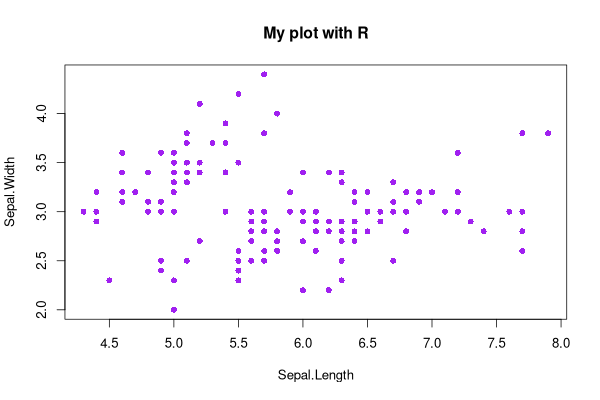
\includegraphics[width=0.6 \textwidth]{figures/scatterplot.png}
\caption{A figure. \label{fig-scatterplot}}
\end{figure}

\section{Discussion}
\label{sec:orge5df4ae}
Lorem ipsum dolor sit amet, consectetuer adipiscing elit.  Donec hendrerit tempor tellus.  Donec pretium posuere tellus.  Proin quam nisl, tincidunt et, mattis eget, convallis nec, purus.  Cum sociis natoque penatibus et magnis dis parturient montes, nascetur ridiculus mus.  Nulla posuere.  Donec vitae dolor.  Nullam tristique diam non turpis.  Cras placerat accumsan nulla.  Nullam rutrum.  Nam vestibulum accumsan nisl.

\section{Conclusion}
\label{sec:org25ce749}
Aliquam erat volutpat.  Nunc eleifend leo vitae magna.  In id erat non orci commodo lobortis.  Proin neque massa, cursus ut, gravida ut, lobortis eget, lacus.  Sed diam.  Praesent fermentum tempor tellus.  Nullam tempus.  Mauris ac felis vel velit tristique imperdiet.  Donec at pede.  Etiam vel neque nec dui dignissim bibendum.  Vivamus id enim.  Phasellus neque orci, porta a, aliquet quis, semper a, massa.  Phasellus purus.  Pellentesque tristique imperdiet tortor.  Nam euismod tellus id erat.

% \nocite{*}% Show all bib entries - both cited and uncited; comment this line to view only cited bib entries;
\bibliography{biblio}%
\end{document}